\documentclass[anon]{CI}
\usepackage[latin1]{inputenc}
\usepackage[english]{babel}

% The following packages will be automatically loaded:
% amsmath, amssymb, natbib, graphicx, url, algorithm2e

\title[CI Project]{Swarm intelligence for counting the degrees of separation in Social Networks}

 % Use \Name{Author Name} to specify the name.
 % If the surname contains spaces, enclose the surname
 % in braces, e.g. \Name{John {Smith Jones}} similarly
 % if the name has a "von" part, e.g \Name{Jane {de Winter}}.
 % If the first letter in the forenames is a diacritic
 % enclose the diacritic in braces, e.g. \Name{{\'E}louise Smith}

 % Two authors with the same address
  % \coltauthor{\Name{Author Name1} \Email{abc@sample.com}\and
  %  \Name{Author Name2} \Email{xyz@sample.com}\\
  %  \addr Address}

 % Three or more authors with the same address:
 % \coltauthor{\Name{Author Name1} \Email{an1@sample.com}\\
 %  \Name{Author Name2} \Email{an2@sample.com}\\
 %  \Name{Author Name3} \Email{an3@sample.com}\\
 %  \addr Address}


 % Authors with different addresses:
 \author{\Name{�lex Pardo Fernandez} \Email{alexpardo.5@gmail.com}\\
 \AND
 \Name{David S�nchez Pinsach} \Email{sdividis@gmail.com}\\
 }

\begin{document}

\maketitle

\begin{abstract}
This is a great project and therefore it has a concise abstract.
\end{abstract}

\begin{keywords}
Swarm Intelligence, Ant Colony Optimization, Twitter, Degrees of Separation.
\end{keywords}


\section{Problem statement and goals} % 1 p�gina

%\textbf{This is where the content of your paper starts. Remember:
%\begin{itemize}
%\item Limit the main text (without bibliography and appendices) to 10 pages.
%\item Include, either in the main text or the appendices, enough details to convince the lecturers of the project's merits.
%\item You should cite all relevant references, including your own.
%\end{itemize}}
\par
One of the most important features of humans and in general, of lots of animals, is the sociability. The ability of communicating each other in order to share knowledge. Human social relationships form a network where everyone is connected with those that communicates often (considered as fiends). 
\\ \par
The theory of the six degrees of separation was originally set out by Frigyes Karinthy \citep{karinthy1929chain} and explains that everyone is connected to any other person in the world by six degrees. That means, if you want to met someone in the world, you will need to pass by other five persons, as maximum, between you and your objective so the last one will be the one you are trying to reach. During these last decades, the six degree theory has been used in many fields like economy, social networks and markets and is a known property of small-world networks where most nodes are not neighbours of one another, but most nodes can be reached from every other by a small number of steps.
\\\par
Twitter is one of the biggest social networks, that is over 200 million users and over 400 million tweets (the 140 character messages that are the main feature of this social network) every day \footnote{Information by March of 2013: \href{https://blog.twitter.com/2013/celebrating-twitter7}{https://blog.twitter.com/2013/celebrating-twitter7}}. The main idea is to create shorts messages of the 140 characters in order to express your ideas or opinions in a shorten way. Moreover, Twitter have introduced some concepts that are very popular now such as the \emph{hash-tag} which is a way of tagging the messages in order to find all the related ones.

Another famous social network is Foursquare, a social network related to places in which you activate the application and notifies your friends that you have been in that place. The most active users in one place achieve some goals such as being the ``major'' of a certain place. Foursquare has over 45 million users and over 3 billion check-ins every day \footnote{Information by January of 2014: \href{https://foursquare.com/about}{https://foursquare.com/about}}.
\\\par
The main objective of this work will be to estimate the degrees of separation in Foursquare and if it is computationally possible, in Twitter and see if it is possible to obtain six degrees of separation between two random people. In order to do this task, it will use some ideas of the Computational Intelligence like Swarm Intelligence. In particular we are going to use Ant Colony Optimization (ACO) \citep{Colorni91} for Shortest Path finding (SPACO) \citep{angus}.



%Content:
%\begin{enumerate}
%\item Explain theory of the 6 degrees
%\item Define the network
%\item Goals: estimate the degrees of separation in twitter
%\end{enumerate}


\newpage

\section{Previous work} % 2 p�gines

The previous work is based on these ideas:
\begin{itemize}
\item ACO original \citep{Colorni91}: Explain the algorithm of the Ant Colony Optimization.
\item General theory \citep{watts}: Explain the general theory about the six degree.
\item On Twitter as \citep{cheng}: Explain the six degree on the Twitter network.
\item On other social nets such as


\end{itemize}

\section{The CI methods} % 3-4 p�gines

Swarm intelligence is a natural method based in the behaviour of the decentralized individuals who obtain solutions in some problem as result of their interactions. These agents normally are simple, with a few capabilities and follow simple rules. It includes ACO, flocking of the birds, bacterial grow or some on. 
\\\\
As it is mentioned previously, we will use the ACO algorithm in order to obtain the degree of separation of two random person in a graph. This algorithm is inspired on the way ants have to solve the problem of finding the best path to achieve a goal such as going from the nest to the found food. The ants cannot communicate with the others and only use the trace of pheromone as a probabilistic method in order to obtain the choice when they have different options. When a ant travels through two points it leaves a few of pheromone on the trail. The other ants around these points feel the pheromone and try to follow this path. The paths with few pheromone will have less probability than the path with high pheromone. As shows the figure \ref{fig:aco}, the path of the ants converge to the shortest path between two points and this is the main characteristic of this method. We will use this idea of the shortest path between two points, as a minimum degree between two person in Foursquare and Twitter networks. In the appendix \ref{implementation}, it will be shown how the algorithm works in details.

\begin{figure}[htb!]
\centering
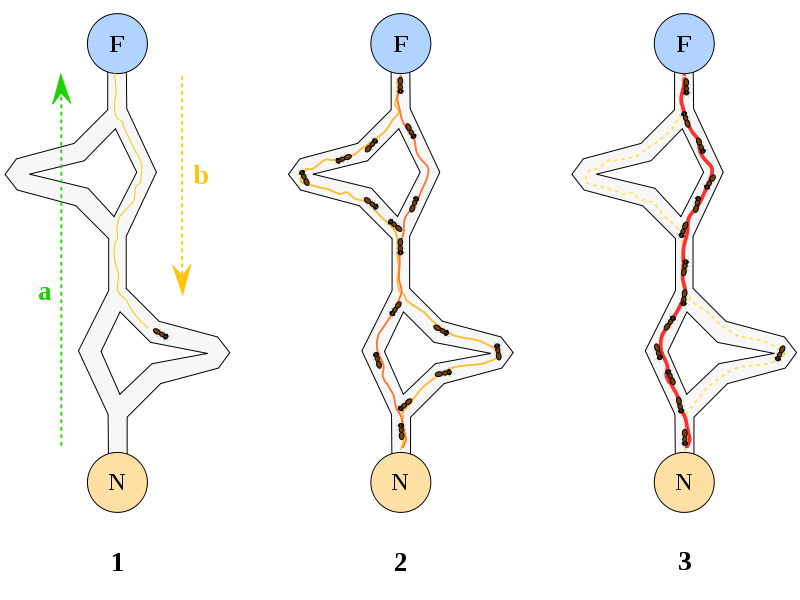
\includegraphics[width=0.6\textwidth]{img/aco}
\caption[ACO algorithm]%
    {ACO algorithm\footnote{Credits to Johann Dr�o, 27 may 2006}}
\label{fig:aco}
\end{figure}

Some considerations needed to take into account are the parameters of the algorithm. These are: the amount of pheromone leaved by each ant, the number of ants of the system, the dissipation of the pheromone and the number of epochs the algorithm will run.

% Amount of pheromone
% - set to 1
% - since weights are always 1, the pheromone is always the same
% - ants returning to the nest (start) leave pheromone also in the trail
% - additionally as \citep{dorigo1999ant} says, the amount of pheromone of the system is kept fixed, so at each iteration it is normalized to always sum a value equal to the number of nodes.


% Number of ants in the system
% - on each epoch, some ants are introduced on the system this allows the new ants to follow the paths started by the ants on the previous epochs
% - as \citep{dorigo1999ant} says, the number of ants should be equal to the number of nodes. Not possible in big graphs such as the Foursquare one, so we reduced the number of ants and increased the number of epochs
% - Once an ant is at distance 15 from the nest, we consider the ant has been lost so we do not follow it anymore (i.e. the ant is deleted from the system) this allows the code to run much more faster since we are only interested in shortest paths.

% Dissipation of the pheromone
% - disipation of pheromone allows the system to forget bad solutions in essence, bad solutions are long so the ants take longer to go from the nest to the food, the disipation allows the ants to explore aditional paths. Shortest paths also suffer the disipation but since are shorter, ants will arrive faster and the disipation will be compensated by the pheromone leaved

% Number of epochs
% - the number of epochs has to be taken into account using the number of ants on the system, the expected lentgh of the path and the computational time associated to the problem.
% - num of ants -> if there are a lot of ants, the system will be slower but will converge earlier, if the number of ants is lower, we will have to increase the number of epochs in order to converge
% - expected length of the path -> the number of epochs is expected to be greatest than the expected length of the shortest path since ants perform one step at each epoch.
% - Computational time -> since we are working with huge graphs (3 million of nodes and 11 million of edges), the computational cost of the algorithm is crucial, and the greatest the number of epochs, the greatests the number of expaned nodes. As explained on \ref{implementation}, the pheromones saved are the ones in which the amount is increased, so when the number of expanded nodes increasesm the ammount of memory needed also increases.

\section{Results and Discussion} % 1-2 p�gines de text

In order to perform the tests we used two different datasets and with different configuration of the execution. Remember as parameters the algorithm have the following:

\begin{table}
	\centering
    \begin{tabular}{l|l}
    \hline
    NUM\_ANTS     & Maximum number of the ants in the system    \\ \hline
    ITERATIONS    & Number of the experiments                   \\ \hline
    DECAY         & Factor of evaporation of the pheromones     \\ \hline
    INCREMENT     & Number of the increment of the pheromones   \\ \hline
    ANTS\_PER\_TURN & Number of ants at each turn that appears    \\ \hline
    MAX\_EPOCH    & Number of the iterations at each experiment \\ \hline
    \end{tabular}
    \caption{Table of the parameters description of the algorithm}
    \label{parameters}
\end{table}

The next table \ref{datasets}, shows the number of the nodes and edges at each dataset.
\begin{table}
	\centering
    \begin{tabular}{l|l|l}
    ~ & Number of the nodes & Number of the edges \\ \hline
    Twitter dataset     & ~                   & ~                   \\ \hline
    Foursquare          & ~                   & ~                   \\ \hline
    \end{tabular}
    \caption{Table of the experimental dataset}
    \label{datasets}
\end{table}

\section{Extensions, strengths and weaknesses}

\section{Conclusions}

\bibliography{bibliography.bib}

\appendix


\section{Implementation details} 
\label{implementation}

The application has been coded using Python 2.7. The system uses NetworkX library in order to represent the graph. Additionally, in order to create an small dataset based on twitter, we used Twython implementation of the Twitter API in order to acquire the data and again, NetworkX in order to save the resulting graph.

We based the code in the next basic pseudo-code algorithm of the ACO:
\\
�put here pseudocode!
\\
Next to the pseudo-code we want to enter a few detail of some parts of the code and how this parts had been coded.
\begin{itemize}
\item \textbf{Pheromone}: The pheromone is the most important part of the our problem and our code. Remember that the ants try to follow the path which contain high quantity of pheromone. However the pheromone effect disappears with the time. For this reason, the algorithm need to define two parameters in order to determine the quantity of the pheromone that leaves the ant and the quantity of the pheromone disappears at each turn.

\item \textbf{Start and final points of the ants}: We select always randomly the start and the final point of the ants using the standard Random methods of the python.
\end{itemize}

\end{document}



%
%@article{Swarm intelligence,
%author = {Wikipedia},
%title = {Swarm intelligence},
%month = January,
%year = {2014},
%url = {http://en.wikipedia.org/wiki/Swarm_intelligence}
%}
%
%@article{Six degrees of separation,
%author = {Wikipedia},
%title = {Six degrees of separation},
%month = December,
%year = {2013},
%url = {http://en.wikipedia.org/wiki/Swarm_intelligence}
%}
